This is the note of the week 1 in the course Machine Learning by Andrew Ng. The course starts with an introduction to Machine Learning, Supervised Learning and Unsupervised Learning. We will go directly into the problem Linear Regression which is a problem in Supervised Learning.
%Supervised Learning It can be a continuous value (\textbf{regression}) or a discrete value (\textbf{classification}).
\section{Linear Regression with One Variable}
Linear regression predicts a real-valued output based on an input value (figure \ref{fig:linReg1}). We discuss the application of linear regression to housing price prediction, present the notion of a cost function, and introduce the gradient descent method for learning.
\begin{figure}[!ht]
\centering
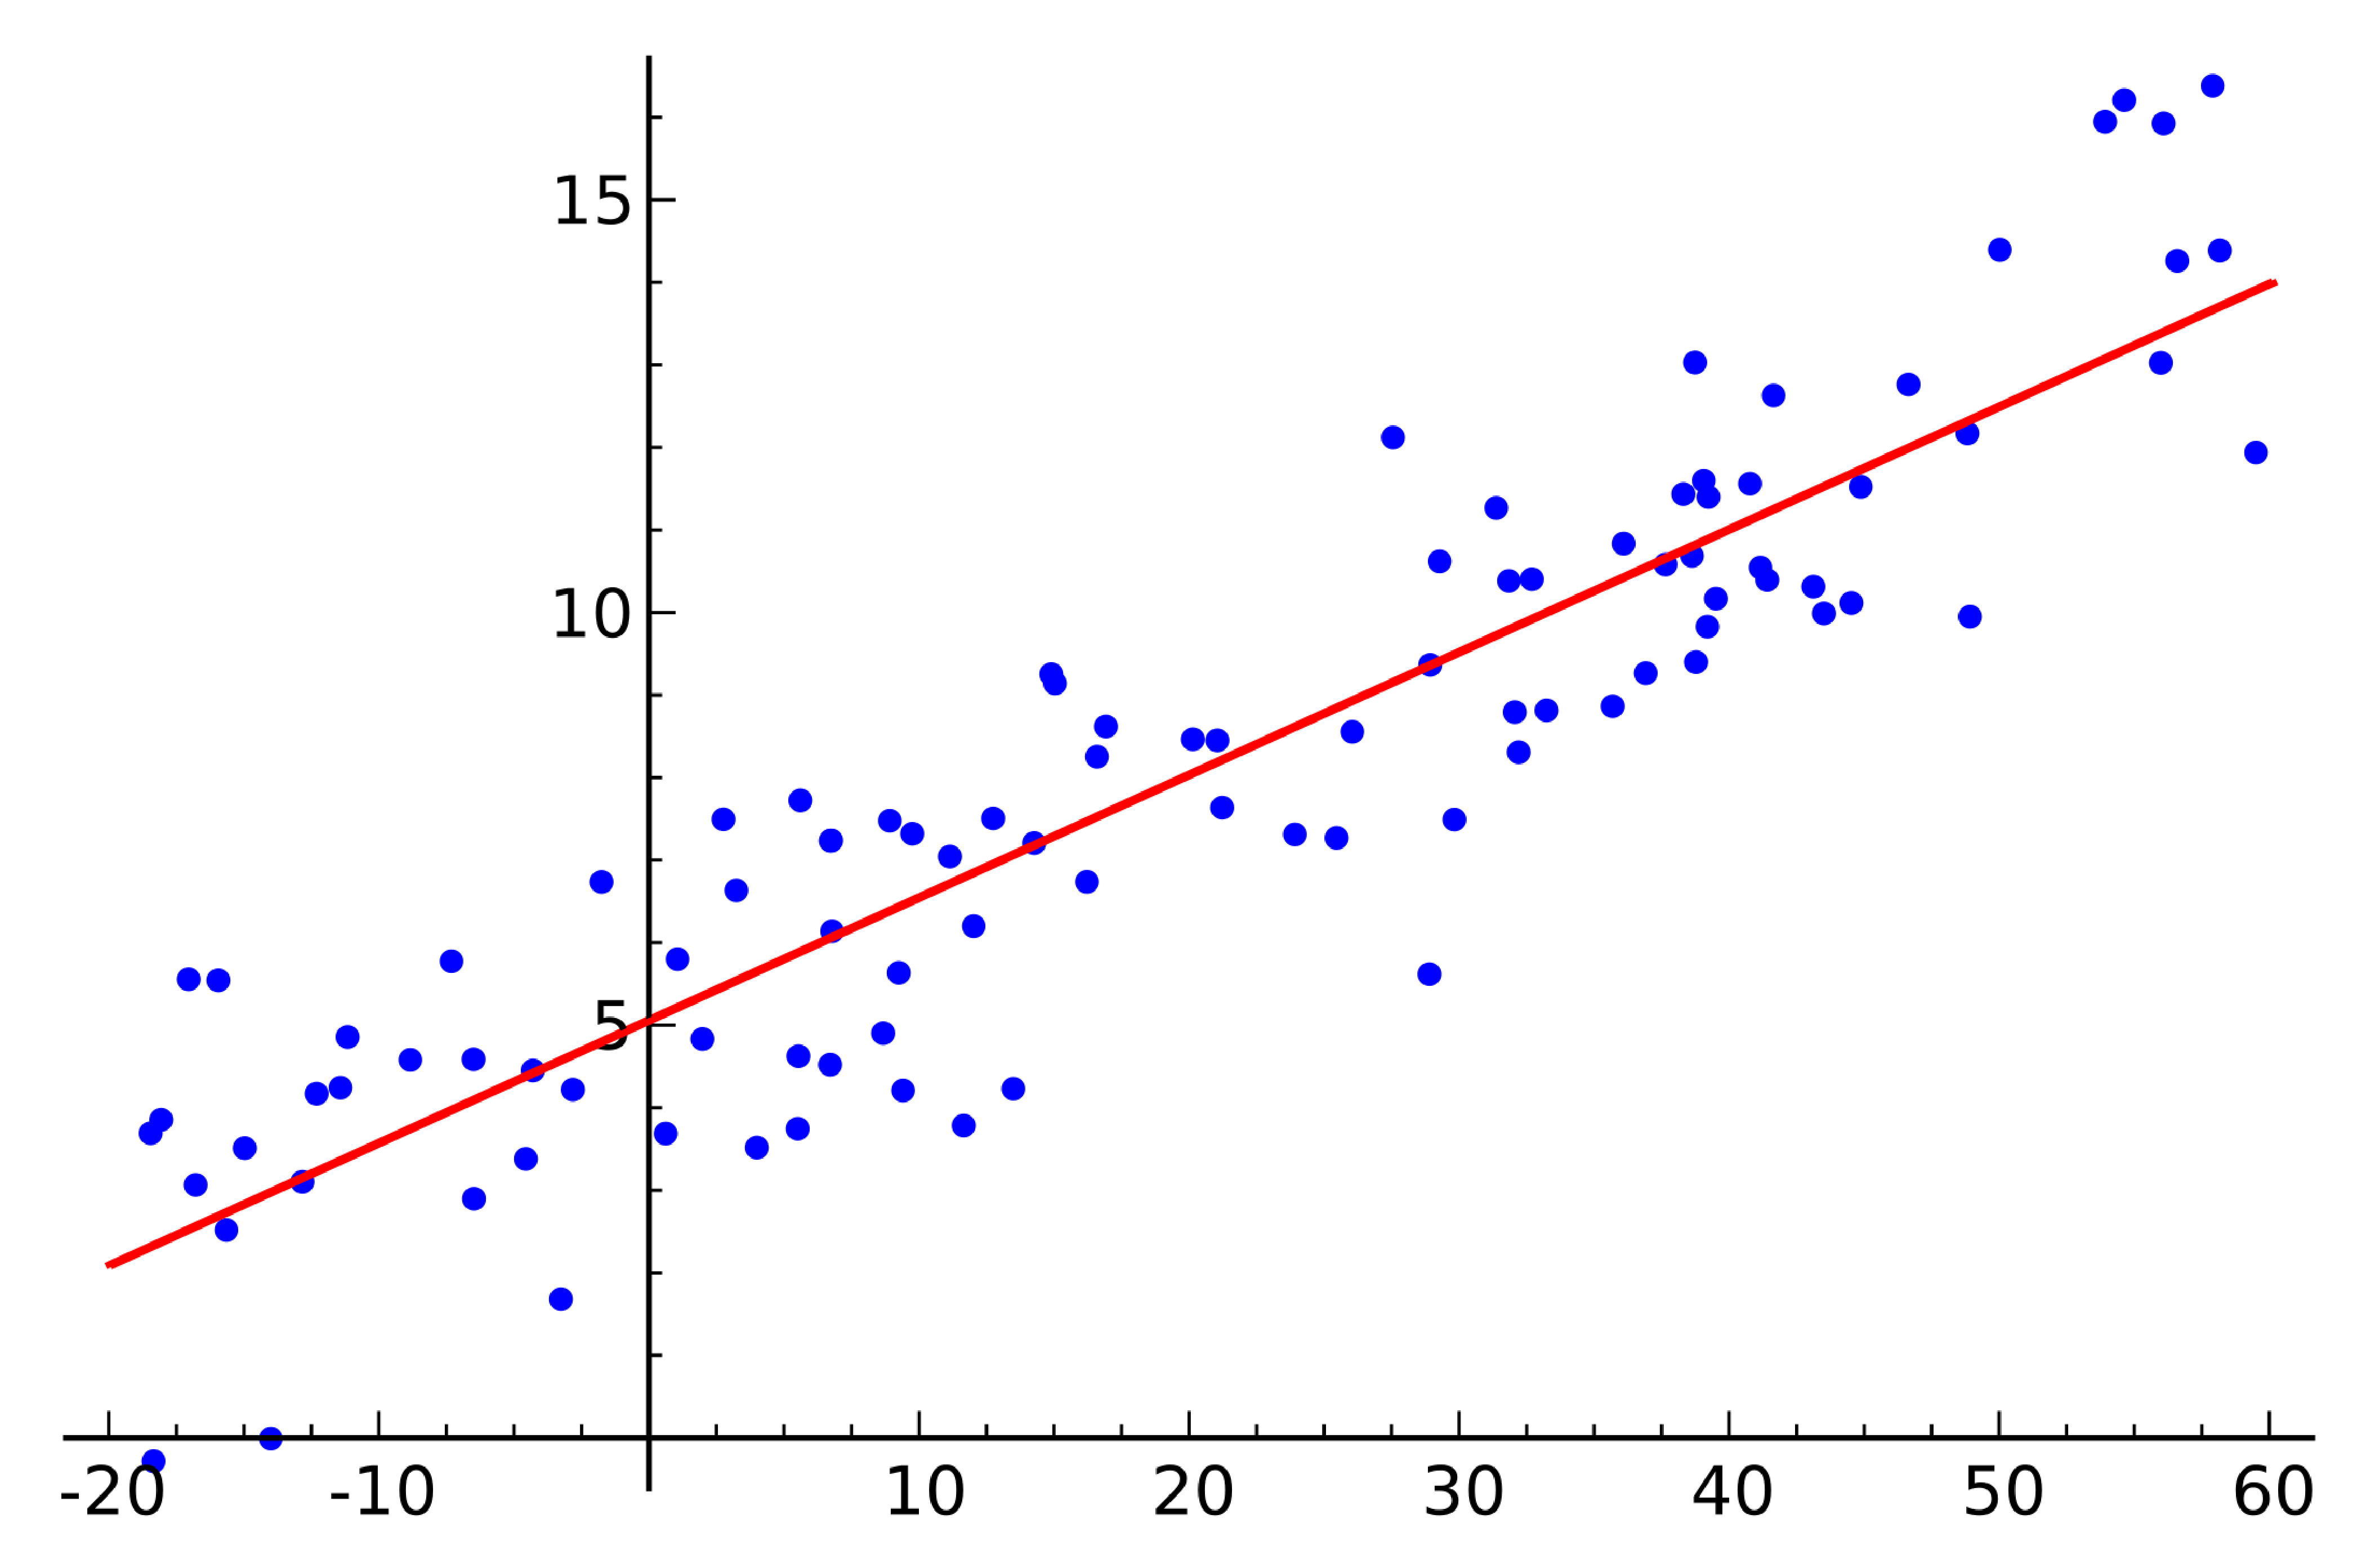
\includegraphics[scale = 0.2]{linReg1.eps}
\caption[Linear Regression]{Based on the red line we can predict a real-valued output for a given input value.}
\label{fig:linReg1}
\end{figure}

\subsection{Model Representation}
Some notation:
\begin{itemize}
	\item $m$ = numbers of training examples
	\item $(x^{(i)}, y^{(i)})$ = the $i^{th}$ training example where $x$ is the input and $y$ is the output 
	\item $h$ = hypothesis function that maps from $x$ to $y$. For example, in figure \ref{fig:linReg1}, $h$ is the red line. We can represent $h$ as following:
	\begin{align}
		h_{\theta}(x) = \theta_{0} + \theta_{1}x  
		\label{form:linReg}
	\end{align}
\end{itemize}
The formula \eqref{form:linReg} is in fact the linear regression with one variable representation (note that $x \in \Re^1$).

\subsection{Cost Function}
In formula \eqref{form:linReg}, how to choose $\theta_0$ and $\theta_1$? The idea is to choose the ones so that $h_{\theta}(x)$ is close to $y$ for our training examples $(x, y)$. We denote $J(\theta_0, \theta_1)$ the cost function. Naturally, we aim to minimize the square errors (which is the cost here) then, the goal is:
\begin{align}
\underset{\theta_0, \theta_1}{\text{minimize}} \; \; J(\theta_0, \theta_1) = \frac{1}{2m}\Sigma_{i = 1}^{m} (h_{\theta}(x^{(i)}) - y^{(i)})^2
\label{form:costFx}
\end{align}
\myaligns{Cost Function}
Note that formula \eqref{form:costFx} contains a factor $\frac{1}{2}$ in order to obtain a factor-free formula after derivative. In addition, the form of this cost function in 3D is always bowl-shaped. It means that if gradient descent method leads us to a local minimum, this is also the global minimum. (see figure \ref{fig:bowlShape}).  
\begin{figure}[!ht]
\centering
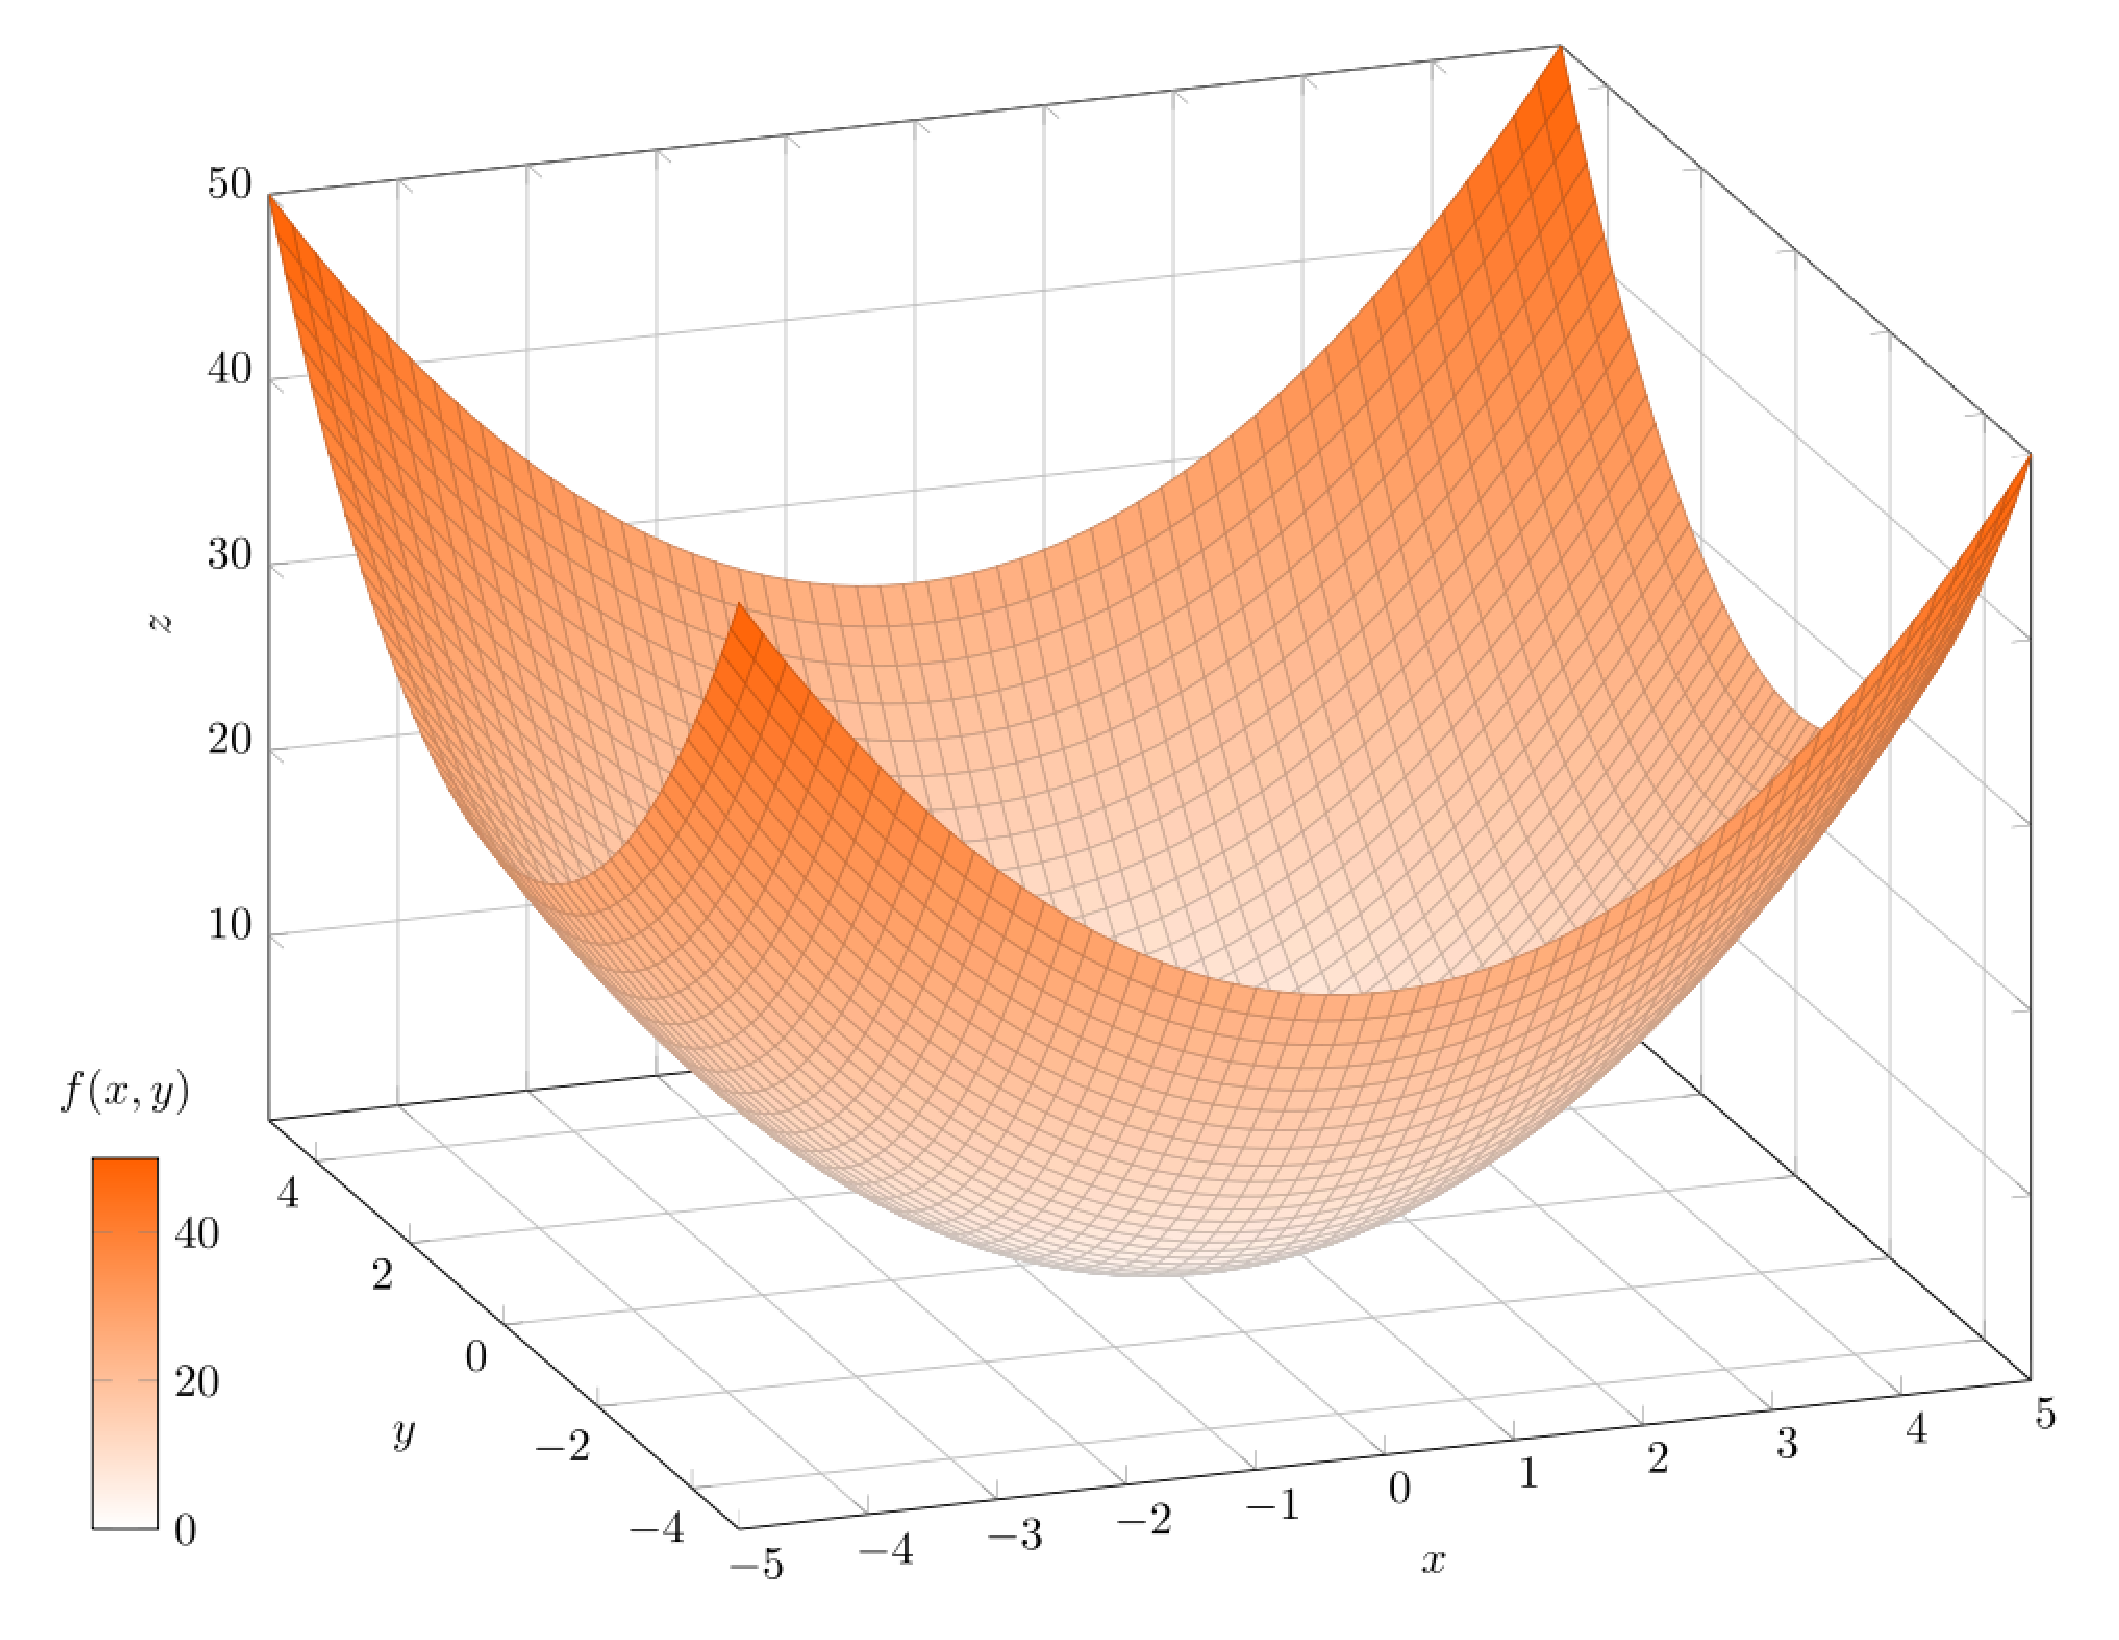
\includegraphics[scale = 0.25]{bowlShape.eps}
\caption[Cost Function Shape]{The 3D-plot of cost function \eqref{form:costFx} is a bowl shape. The horizontal surface is the plane of $(\theta_0, \theta_1)$.}
\label{fig:bowlShape}
\end{figure}

\subsection{Gradient Descent Method}
To solve the problem in formula \eqref{form:linReg}, we can use the Gradient Descent method: For a learning rate $\alpha > 0$ small enough, and a given initial values of $(\theta_0, \theta_1)$, simultaneously update $(\theta_0, \theta_1)$ as following:
\begin{align}
\label{form:gradDesc}
temp0 &:= \theta_0 - \alpha \frac{\partial J(\theta_0, \theta_1)}{\partial \theta_0} \nonumber \\
temp1 &:= \theta_1 - \alpha \frac{\partial J(\theta_0, \theta_1)}{\partial \theta_1} \\
\theta_0 &:= temp0 \nonumber\\
\theta_1 &:= temp1 \nonumber
\end{align}

Figure \ref{fig:gradDesc} illustrates how gradient descent work: it will start from an initial values and then go to the local minimum (in this case it's also the global minimum). I can prove (in an intuitive way) like this: Set $\theta_{j}' = \theta_j - \alpha \frac{\partial J}{\partial \theta_j}$ with $\alpha$ positive and small enough such that $\frac{J(\theta_{j}') - J(\theta_j)}{\theta_{j}' - \theta_j} \approx \frac{\partial J}{\partial \theta_j}$. Now for both case when $\frac{\partial J}{\partial \theta_j} > 0$ or $\frac{\partial J}{\partial \theta_j} < 0$, we can easily prove that $J(\theta_{j}') < J(\theta_j)$. Hence, it leads to a local minimum. Note that the fact $\alpha$ is small enough is critical because otherwise it will not be approximative to the derivative. We can also solve  analytically the problem \eqref{form:costFx} but Gradient Descent method is good for scaling, i.e. it works well with big input data.  
\begin{figure}[!ht]
\centering
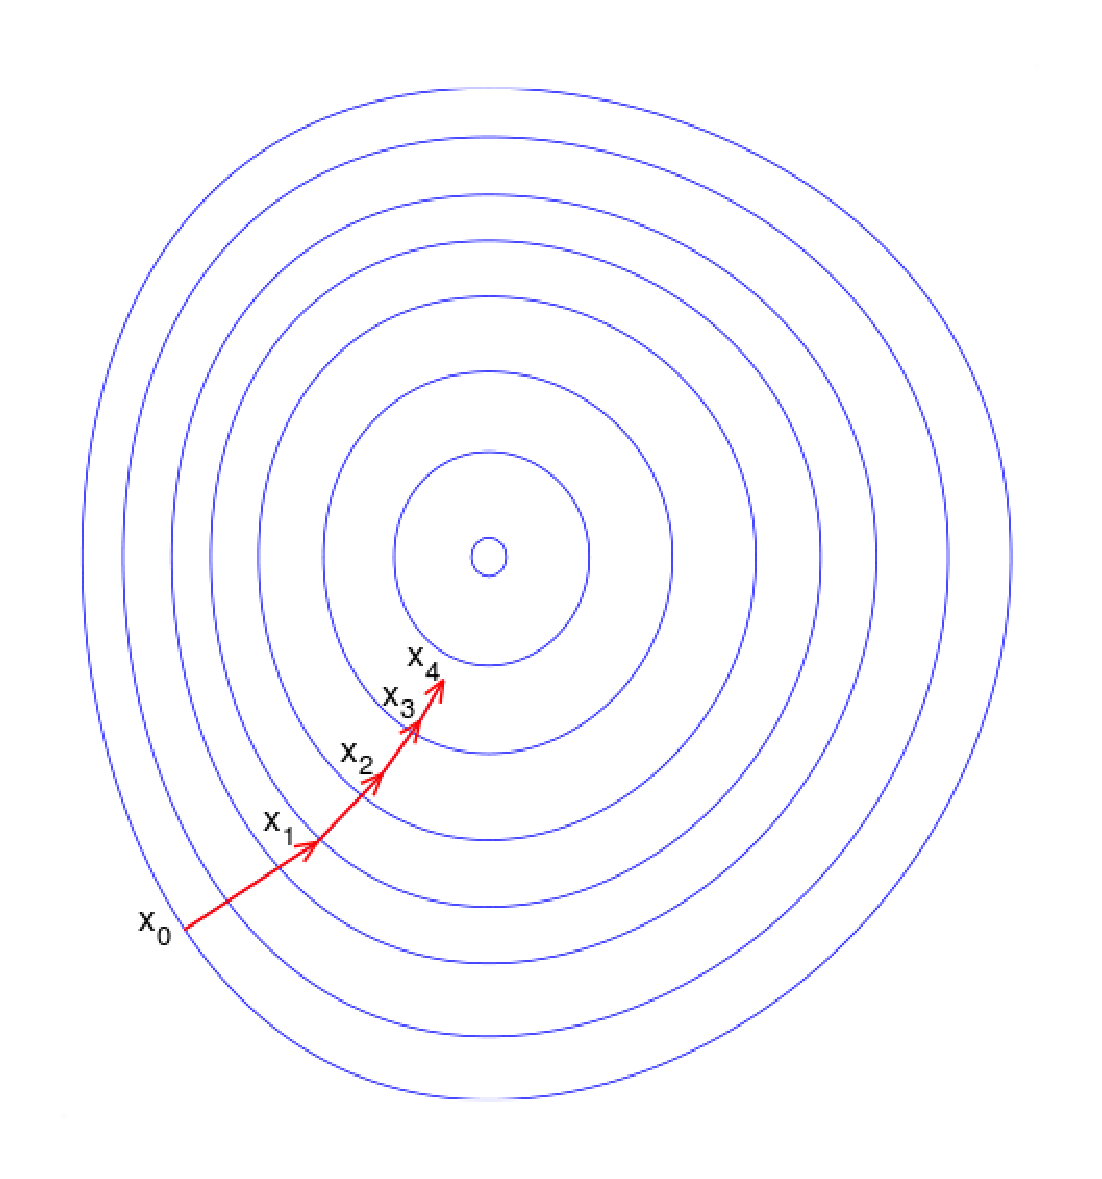
\includegraphics[scale = 0.3]{gradDesc.eps}
\caption[Gradient Descent Illustration]{The circles are the contour plots of intersection between horizontal surfaces with 3D-plot of cost function. It means that the points (i.e. a point = $(\theta_0, \theta_1)$) lie on same circle has equals cost.}
\label{fig:gradDesc}
\end{figure}

From \eqref{form:linReg}, \eqref{form:costFx} and \eqref{form:gradDesc}, we have the explicit assignment in \eqref{form:finalGradDesc}:
\begin{align}
\label{form:finalGradDesc}
\theta_0 &:= \theta_0 - \alpha \frac{1}{m} \Sigma_{i=1}^{m} (h_{\theta}(x^{(i)}) - y^{(i)}) \nonumber \\
\theta_1 &:= \theta_1 - \alpha \frac{1}{m} \Sigma_{i=1}^{m} (h_{\theta}(x^{(i)}) - y^{(i)})x^{(i)} 
\end{align}
\myaligns{Univariate Gradient Descent}